%%%%%%%%%%%%%%%%%%%%%%%%%%%%%%%%%%%%%%%%%%%%%%%%%%%%%%%%%%%%%%%%%
% Lecture date: 19-12-09
%%%%%%%%%%%%%%%%%%%%%%%%%%%%%%%%%%%%%%%%%%%%%%%%%%%%%%%%%%%%%%%%%
\chapter{Electroweak Processes}
We will consider $\SU(2)_\text{L} \times \Uni(1)_\text{Y}$ theory.

\section{Muon decay}
$V-A$ interaction

\begin{align*}
   \feynmandiagram[horizontal=i1 to v1, medium, layered layout]{
      i1[particle=\(\mu\)] --[momentum=\(p\), fermion]v1,
      v1 --[momentum=\(k_1\), fermion] f3[particle=\(\nu_\mu\)],
      v1 -- [photon, edge label=\(W\)] v2,
      {[same layer] v2, f3},
      v2 --[fermion, momentum=\(k_2\)] f1[particle=\(e^-\)],
      v2 --[anti fermion, momentum=\(k_3\)] f2[particle=\(\bar\nu_e\)],
      {[same layer] f1, f2},
   };
\end{align*}

$q = k_2 + k_3 = p - k_1$
\begin{align*}
   i \M = \overline{u}(k_1)  \frac{-ig}{\sqrt{2}} \gamma^\mu P_L u(p) \frac{-ig_{\mu\nu}}{q^2 - M_W^2} \overline{u}(k_2) \frac{-ig}{\sqrt{2}} \gamma^\nu P_L v(k_3)
\end{align*}

In spinor space, Dirac equation 
\begin{align}
   (\slashed{p} - m) u(p) = 0.
\end{align}

Propagator $M_W \sim \SI{80}{\giga\eV}$ and $m_\mu = \SI{100}{\mega\eV}$, i.e.~$p^2 \ll M^2$. So $4$-Fermi approximation is obtained.
\begin{align*}
   \frac{1}{q^2 - M_W^2} = - \frac{1}{M_W^2} \frac{1}{1 - q^2 / M_W^2} \approx -\frac{1}{M_W^2}
\end{align*}
Then the coupling is effectively
\begin{align}
   G_F = \frac{\sqrt{2} g^2}{8 M_W^2}
\end{align}
Note that when for example top and bottom quarks are present, this approximation is not valid any more.

Proceed with $m_e = m_{\nu_e} = m_{\nu_\mu} = 0$
\begin{align*}
   \M &= -\frac{4G_F}{\sqrt{2}} \overline{u}(k_1) \gamma^\mu P_L u(p) \overline{u}(k_2) \gamma_\mu P_L v(k_3) \\
   \frac{1}{2} \sum_{\text{spins}} |\M|^2 &= \frac{16 G_F^2}{2 \cdot 2} \overline{u}(k_1) \gamma^\mu P_L u(p) \overline{u}(p) P_R \gamma^\nu u(k_1) \overline{u}(k_2) \gamma_\mu P_L v(k_3) \overline{v}(k_3) P_R \gamma_\nu u(k_2) \\
                                          &= 4 G_F^2 \tr[\slashed{k}_1 \gamma^\mu P_L (\slashed{p} + m_\mu) P_R \gamma^\nu] \cdot \tr[\slashed{k}_2 \gamma_\mu P_L \slashed{k}_3 P_R \gamma_\nu]
                                          \shortintertext{Term with $m_\mu$ vanishes, since $P_L P_R = 0$}
\end{align*}

Computing the two traces
\begin{align*}
   \tr[\slashed{k}_1 \gamma^\mu \slashed{p}\gamma^\nu P_L] &= \frac{4}{2}  \left( k_1^\mu p^\nu - k_1 p g^{\mu\nu} + k_1^\nu p^\mu \right) - \frac{4i}{2} \epsilon_{\alpha\mu\beta \nu} {k_1}_\alpha p_\beta  \\
   \tr[\slashed{k}_2 \gamma_\mu \slashed{k}_3 \gamma_\nu P_L] &= \frac{4}{2}  \left( (k_2)_\mu (k_3)_\nu - k_2 k_3 g_{\mu\nu} + {k_2}_\nu {k_3}_\mu \right) + \frac{4i}{2} \epsilon \epsilon_{\alpha \mu \beta \nu} k_2^\alpha k_3^\beta
\end{align*}
Using the fact that $\epsilon$ is totally anti-symmetric tensor, so the terms with one $\epsilon$ sum to zero. Note further
\begin{align}
   \epsilon^{\mu\nu\rho\sigma} \epsilon_{\mu\nu}^{\quad \rho'\sigma'} = -2 (g^{\rho \rho'}g^{\sigma \sigma'} - g^{\rho\sigma'} g^{\rho'\sigma})
\end{align}

In order to use this formula
\begin{align*}
   &\sigma^{\alpha \mu \beta \nu} \sigma_{\alpha' \mu \beta' \nu} \\
   &= \epsilon^{\mu \nu \alpha \beta} \epsilon^{\quad \alpha'' \beta''}_{\mu\nu} g_{\alpha' \alpha ''} g_{\beta ' \beta''} \\
   &= (-2) \left[ g^{\alpha \alpha''} g^{\beta \beta''} - g^{\alpha \beta''} g^{\beta \alpha''}\right] g_{\alpha' \alpha''} g_{\beta' \beta''} \\
   &= (-2) \left[ \delta^{\alpha}_{\alpha'} \delta^{\beta}_{\beta'} - \delta^{\alpha}_{\beta'} \delta^{\beta}_{\alpha'}  \right]
\end{align*}

Terms without $\epsilon$
\begin{align*}
   &4 (k_1^\mu p^\nu + k_1^\nu p^\mu - g^{\mu\nu} k_1 \cdot p) (k_{2 \mu} k_{3 \nu} + k_{2\nu} k_{3\mu} - k_2 \cdot k_3 g_{\mu\nu}) \\
   &= \dots = 4 \left[ 2 (k_1 \cdot k_2) (p\cdot k_3) + 2 (k_1\cdot k_3)( p \cdot k_2) \right] \\
   &= 8 \left[ (k_1 \cdot k_2)( p \cdot k_3) + (k_1 \cdot k_3) (p \cdot k_2) \right]
\end{align*}

Then
\begin{align*}
   \frac{1}{2} \sum_{\text{spins}} |\M|^2 = 64 G_F^2 (k_1 \cdot k_2)( p\cdot k_3)
\end{align*}
Recall
\begin{align}
   \begin{split}
   \dd{\Gamma} &= \frac{1}{2E} \overline{|\M|^2} \dd{Q} \\
   \dd{Q} &= \frac{\dd[3]{k_1}}{(2\pi)^3 2 E_{k_1}} \frac{\dd[3]{k_2}}{(2\pi)^3 2 E_{k_2}} \frac{\dd[3]{k_3}}{(2\pi)^3 2 E_{k_3}} (2\pi)^{4} \delta^{(4)} (p-k_1 -k_2 - k_3)
   \end{split}
\end{align}

One can prove (In \sm neutrino has no mass.)
\begin{align}
   \frac{\dd[3]{k_1}}{(2\pi)^3 2 E_{k_1}} = \int \dd[4]{k_1} \theta(E_1) \delta(k_1^2)
\end{align}

Use identity of Delta function involving composite function.
\begin{align*}
   \frac{\dd[3]{k_1}}{(2\pi)^3 2 E_{k_1}} \delta^{(4)}(p- k_1 -k_2 - k_3 ) = \int \dd[4]{k_1} \theta(E_1) \delta(k_1^2) \delta^{(4)}(p- k_1 -k_2 - k_3 ) \\
   = \theta(k_1)\delta^{k_1^2}
\end{align*}

Thus 
\begin{align*}
   \dd{Q} = \frac{1}{(2\pi)^5} \frac{\dd[3]{k_2}}{2E_{k_2}} \frac{\dd[3]{k_3}}{2E_{k_3}} \theta(E - E_{k_2} - E_{k_3}) \delta((p-k_2-k_3)^2)
\end{align*}

In rest frame of muon 
$p \cdot k_3 = m_\mu \cdot E_3$
\begin{align*}
   (k_1 + k_2)^2 &\approx 2 k_1 \cdot k_2 \\
   k_1 \cdot k_2 &\approx \frac{1}{2} (k_1 + k_2)^2 \\
                 &= \frac{1}{2} (p-k_3)^2 \\
                  &= \frac{1}{2} \left[ p^2 - 2 p\cdot k_3 + k_3^2 \right] \\
                  &= \frac{1}{2} [m_\mu^2 - 2 m_\mu E_3]
\end{align*}

\begin{align*}
   \frac{1}{2} \overline{|\M|^2} &= 64 G_F^2 k_1\cdot k_2 p \cdot k_3 \\
   &= 64 G_F^2 m_\mu E_3 [m_\mu^2 - 2 m_\mu E_3]
\end{align*}
Now we have computed $|\M|^2$, the actual difficulties are in phase space integral. For $n$-particle phase space, often use Monte-Carlo integration technique.

With $\theta$ the angle between electron and electron neutrino ($k_2$ and $k_3$)
\begin{align*}
   (p-k_2 - k_3)^2 = p^2 + k_2^2 + k_3^2 - 2 p \cdot k_2 -2 p\cdot k_3 + 2k_2 \cdot k_3 \\
   = m_\mu^2 - 2 m_\mu E_2 - 2m_\mu E_3 + 2 E_2 E_3 (1-\cos \theta)
\end{align*}

\begin{align*}
   \dd[3]{k_2} \dd[3]{k_3} = (4\pi) (2\pi) E_2^2 \dd{E_2} E_3^2 \dd{E_3} \dd{\cos \theta}
\end{align*}

\begin{align*}
   \delta(\dots - 2 E_2 E_3 \cos \theta) = \frac{1}{2E_2 E_3} \delta(- \cos \theta)
\end{align*}

\begin{align*}
   \dd{\Gamma} = \frac{G_F^2}{2 \pi^3} \dd{E_3} \dd{E_3} E_3 (m_\mu^2 - 2 m_\mu E_3)
\end{align*}

\begin{align*}
   \frac{1}{2} m_\mu - E_2 \leq E_3 \leq \frac{1}{2} m_\mu \\
   0 \leq E_2 \leq \frac{1}{2} m_\mu
\end{align*}

Carrying the integration out
\begin{align*}
   \frac{\dd{\Gamma}}{\dd{E_2}} &= \frac{m_\mu G_F^2}{2\pi^3} \int_{\frac{1}{2}m_\mu - E_2}^{\frac{1}{2}m_\mu} \dd{E_3} E_3 (m_\mu - 2 E_3) \\
                                &= \frac{G_F^2}{2\pi^3} m_\mu^2 E_2^2 \left( 3 - \frac{4E_2}{m_\mu} \right)
\end{align*}

Finally
\begin{align*}
   \Gamma = \frac{1}{\tau_\mu} = \int^{\frac{1}{2}m_\mu}_0 \dd{E_2} \frac{\dd{\Gamma}}{\dd{E_2}} = \frac{G_F^2 m_\mu^5}{192 \pi^3}
\end{align*}
If $m_e \neq 0$
\begin{align*}
   \Gamma = \frac{1}{\tau_\mu} = \int^{\frac{1}{2}m_\mu}_0 \dd{E_2} \frac{\dd{\Gamma}}{\dd{E_2}} = \frac{G_F^2 m_\mu^5}{192 \pi^3} \left[ 1 - 8r^2 + 8r^6 - r^8 - 24 r^4 \ln{r} \right]
\end{align*}
with $r = m_e / m_\mu$. $r$ enters in boundary of phase space integration.
%%%%%%%%%%%%%%%%%%%%%%%%%%%%%%%%%%%%%%%%%%%%%%%%%%%%%%%%%%%%%%%%%
% Lecture date: 19-12-16
%%%%%%%%%%%%%%%%%%%%%%%%%%%%%%%%%%%%%%%%%%%%%%%%%%%%%%%%%%%%%%%%%

If one tries to measure the decay width precisely, the $1$-loop electroweak correction must also be included.
%TODO: diagram
\begin{align*}
   \includegraphics[width=0.5\linewidth]{muonDecay/1.eps}
\end{align*}

Neutrino can also be considered in the calculation and one finds an upper bound for neutrino mass $m_{\nu_\mu} \leq \SI{1}{\kilo \eV}$.

Mass dimension of $\Gamma$ is $+1$. Using dimensional argument, since $[G_F] = -2$, the decay width $\Gamma \sim G_F^2 m_\mu^5$. Grand Unified Theory postulates the decay of proton, $p \rightarrow e^+ \pi^0$. Following $M_{X,Y} \sim \SI{10e16}{\giga \eV}$, we estimate the decay width of proton $\Gamma \sim \frac{g_{\mathbf{SU}(5)}^4}{M_X^4} M^5_{p}$.
\begin{align*}
   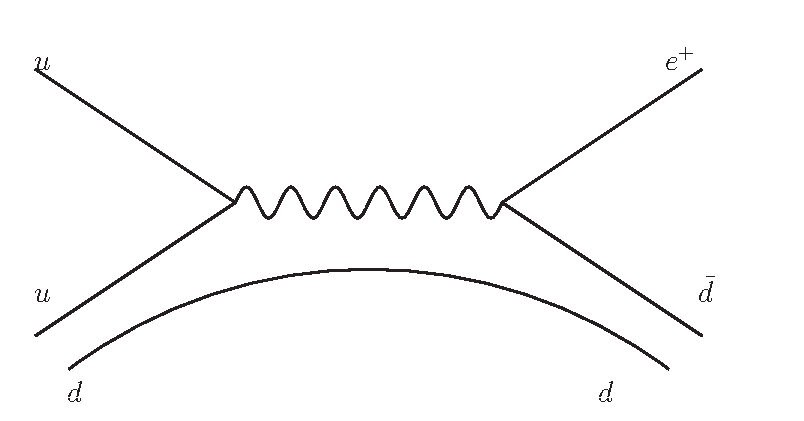
\includegraphics[width=0.5\linewidth]{muonDecay/2.eps}
\end{align*}

\paragraph{Polarized Muon Decay}
In the above computation, the muon polarizations are summed over. Assume the polarization is fixed
% TODO: diagram. helicity and angular momentum conservation

Also the spin sum relation enables us the computation. How to compute decay of polarized particle then? Recall that $u$, $\bar{u}$, $v$ and $\bar{v}$ are independent solutions to Dirac equation.
\begin{align}
   u^{(s)} = \sqrt{E+m} \begin{pmatrix} \chi^{(s)} \\ \frac{\pmb{\sigma} \cdot \pmb{p}}{E+m} \chi^{(s)} \end{pmatrix}
\end{align}
To get chiral-left part of $u^{(s)}$ $P_L u^{(s)}(\pmb{p})$. Can also define two projection operators
\begin{align}
   \Lambda_+ &= \frac{1}{2m} (\slashed{p} + m) \\
   \Lambda_- &= \frac{1}{2m} (-\slashed{p} + m)
\end{align}

They are indeed projection operators
\begin{align*}
   \Lambda_+ + \Lambda_- &= \id_4 \\
   (\Lambda_+)^2 &= \frac{1}{4m^2} \left( \slashed{p} \slashed{p} + 2m \slashed{p} + m^2 \right) = \frac{1}{4m^2} 2m (\slashed{p} + m) = \Lambda_+ \\
   (\Lambda_-)^2 &= \Lambda_-
\end{align*}

Let $\sum_{r=1}^{4} a_r u^{(r)}$ be an arbitrary spinor
\begin{align*}
   \Lambda_+ &= \sum_{r=1}^{4} a_r u^{(r)} \\
             &= \sum_{r=1}^{4} a_r \left( \sum_{s=1}^{2} \frac{u^{(s)}\bar{u}^{(s)}}{2m} \right) u^{(r)}
   \shortintertext{use $\bar{u}^{(s)} u^{(r)} = 2m \delta^{rs}$}
             &= \sum_{r=1}^2 a_r u^{(r)}
\end{align*}
arbitrary $E > 0$ spinor. Thus $\Lambda_+$ projects to $E > 0$ states and $\Lambda_-$ projects $E<0$ states.

Particle at rest, spin $\pmb{s}$ and $|\pmb{s}|=1$. Write a four-vector $s^\mu = (0, \pmb{s})$. At rest $p^\mu = (m, 0)$ and $(s\cdot p) = 0$. 

Starting from the $s^\mu$, can compute $s'^\mu$ in any frame by a Lorentz boost.
\begin{align*}
   s^0 &= \frac{\pmb{p} \cdot \pmb{\xi}}{m} \\
   s^i &= \xi^i + \frac{(\pmb{p} \cdot \pmb{\xi})}{m(m+E)}p^i
\end{align*}
$\pmb{\xi}$ denotes the direction of spin and $|\pmb{\xi}| = 1$

Compute $s \cdot p$ in new frame
\begin{align*}
   s \cdot p &= \frac{\pmb{p} \cdot \pmb{\xi}}{m} E - \pmb{p} \cdot \pmb{\xi} \\
             &= \frac{\pmb{p}\cdot \pmb{\xi} \pmb{p}^2}{m (m+E)} \\
             &= \pmb{p} \cdot \pmb{\xi} \left[ \frac{E}{m} - 1 - \frac{\pmb{p}^2}{m(m+E)} \right] \\
             &=\frac{\pmb{p} \cdot \pmb{\xi}}{ m(m+E)}  \left[ E (m+E) - m(m+E) - \pmb{p}^2 \right] \\
             &= 0
\end{align*} 

Define two projection operators
\begin{align*}
   \Sigma_{\pm} &= \frac{1}{2} \left( \id_4 \pm \gamma^5 \slashed{s} \right) \\
   \Sigma_+ + \Sigma_- &= \id_4 \\
   (\Sigma_-)^2 &= \frac{1}{4} (\id - \gamma^5 \slashed{s}) (\id - \gamma^5 \slashed{s}) \\
                &= \frac{1}{4} \left[ \id - 2 \gamma^5 \slashed{s} + \gamma^5 \slashed{s} \gamma^5 \slashed{s} \right]  \\
                &= \frac{1}{4} [ 2 \id - 2 \gamma^5 \slashed{s}] \\
                &= \Sigma_- \\
   (\Sigma_+)^2 &= \Sigma_+
\end{align*}

What do $\Sigma_\pm$ project out? In rest frame $\Sigma_- = \frac{1}{2} (\id - \gamma^5 \gamma^i s^i)$. Choose $\pmb{s} = \pmb{e}_3 = \pmb{e}_z$. 
\begin{align*}
   \Sigma_- &= \frac{1}{2} (\id - \gamma^5 \gamma^3) \\
            &= \frac{1}{2} \left[ \begin{pmatrix} \id_2 & 0 \\ 0 & \id_2\end{pmatrix}  - \begin{pmatrix} 0 &\id \\ \id & 0 \end{pmatrix} \begin{pmatrix} 0 & \sigma^3 \\ -\sigma^3 & 0 \end{pmatrix}\right] \\
            &= \frac{1}{2} \begin{pmatrix} \id_2 - \sigma^3 & 0 \\ 0 & \id_2 + \sigma^3 \end{pmatrix}
\end{align*}
so project out helicity states.

\begin{align}
   u^k(\pmb{p},s) \bar{u}_i ( \pmb{p}, s) = \frac{1}{2} \left[ (\slashed{p}+ m) (\id - \gamma^5 \slashed{s}) \right]_i^k
\end{align}
or in computation
\begin{align}
   (\slashed{p} + m ) \mapsto \frac{1}{2} (\slashed{p} + m_\mu) (\id - \gamma^5 \slashed{s}_\mu)
\end{align}

Turns out we can skip computation. Replace $p_\alpha \mapsto p_\alpha- m s_\alpha$ in final answer
\begin{align*}
   &\tr[\dots P_R (\slashed{p} + m_\mu) (\id -\gamma^5 \slashed{s}) \gamma_\alpha P_R \dots ] \\
   &= \tr \left[ \dots P_R (\slashed{p} - m_\mu \gamma^5 \slashed{s}) \gamma_\alpha P_R \dots \right] \\
   &= \tr \left[ \dots P_R (\slashed{p} - m \slashed{s}) \gamma_\alpha P_R \right]
\end{align*}
with
\begin{align*}
   \pmb{\xi} \cdot \frac{\pmb{p}_e}{|\pmb{p}_e|} = \cos \theta
\end{align*}
In the end
\begin{align}
   \frac{\dd{\Gamma}}{\Gamma} = \frac{1}{2} \left(1-\frac{1}{3}\cos \theta \right) \dd{\cos \theta}
\end{align}

\section{Nuclear $\beta$-decay}
${}^{14}O \rightarrow {}^{14}N^* e^+ \nu_e$ $\beta^+$-emitter
$n \rightarrow p e^- \bar{\nu}_e$

Non-relativistic limit of Pauli-Dirac spinor
\begin{align*}
   u^{(s)}(\pmb{p}) &= \sqrt{E+m} \begin{pmatrix} \chi^{(s)} \\ \frac{\pmb{\sigma}\cdot \pmb{p}}{E + m} \chi^{(s)}\end{pmatrix} \\
   &\rightarrow \sqrt{2m} \begin{pmatrix} \chi^{(s)} \\ 0 \end{pmatrix}\\
   \bar{u}^{(s)} &= \sqrt{2m} \begin{pmatrix} x^{(s)} & 0\end{pmatrix}
\end{align*}

\begin{align*}
   &\bar{\psi}_n \gamma_\mu \frac{1}{2} \left( \id - \gamma^5 \right) \psi_p (x)
   \shortintertext{$\gamma^5$ matrice has no effect and vanishes}
   &= \frac{1}{2} \bar{\psi}_n (x) \gamma_\mu \psi_p (x) \\
   &= \frac{1}{2} \psi_n (x) \gamma^0 \gamma_\mu \psi_p (x) \\ 
   &\rightarrow  \frac{1}{2} \psi_n^\dagger \psi_p
\end{align*}

$\mu \rightarrow i=1,2,3$
\begin{align*}
   \gamma^0 \gamma^i &= \begin{pmatrix} \id_2 & 0 \\ 0 & -\id_2 \end{pmatrix} \begin{pmatrix} 0 & \sigma_i \\ -\sigma_i & 0 \end{pmatrix}\\
   &= \begin{pmatrix} 0 & \sigma_i \\ \sigma_i & 0 \end{pmatrix}
\end{align*}
It is off-diagonal.

Thus in the non-relativistic limit
\begin{align*}
   \psi_n&^\dagger \gamma^0 \gamma^i \psi_p \rightarrow 0
\end{align*}

%%%%%%%%%%%%%%%%%%%%%%%%%%%%%%%%%%%%%%%%%%%%%%%%%%%%%%%%%%%%%%%%%
% Lecture date: 19-12-17
%%%%%%%%%%%%%%%%%%%%%%%%%%%%%%%%%%%%%%%%%%%%%%%%%%%%%%%%%%%%%%%%%
Typical $\Delta E = \order{\SI{10}{\mega \eV}}$ or so. Thus we can make the approximation $\frac{1}{q^2 - M_W^2} \rightarrow - \frac{1}{M_W^2}$.

Consider transition amplitude in $x$-space
\begin{align*}
   T_{fi} &= -i \frac{4 G_F}{\sqrt{2}} \int \dd[4]{x} J_\mu^{(n)\dagger} J^{(e)\mu}_{(x)}  \\
         &= -i \frac{4G_F}{\sqrt{2}} \int \dd[4]{x} \left[ \bar{\psi}_n (x) \gamma_\mu P_L \psi_p(x) \right] \left[ \bar{\psi}_\nu (x) \gamma^\mu P_L  \psi_e(x) \right]
\end{align*}

Usually, consider $x$-integral immediately, $\rightarrow u, \bar u, v, \bar v$. Defs for now, more convenient due to non-relativistic nature.

Since $J^P = 0^+$ for initial and final states ${}^{14}O$ and ${}^{14}N^*$, no parity change and $\gamma^5$ has odd parity. Thus $\bar{\psi}_n \gamma^\mu \gamma^5 \psi_p$ doesn't contribute.

Assume nuclear wave function is unchanged by transition. $\Delta E \simeq \SI{2}{\mega \eV} \ll m_p, m_n; m_O, m_N$.

Use non-relativistic spinors for $p$ and $n$
\begin{align*}
   \bar{\psi}_n (x) \gamma_\mu \frac{1}{2} (\id - \gamma^5) \psi_p (x)
   \shortintertext{drop $\gamma^5$ and $\mu=0$}
   \rightarrow \frac{1}{2} \psi_n^\dagger (x) \psi_p (x)
\end{align*}

\begin{align*}
   T_{fi} \simeq -i \frac{G_F}{\sqrt{2}} \int \dd[4]{x} \left[ \psi^\dagger_n (x) \psi_p (x) \right] \left[ \bar{\psi}_\nu (x) \gamma^0 (1-\gamma^5) \psi_e (x) \right]
\end{align*}
The wave functions for proton and neutron vanish outside of nuclei, thus the integral is effectively bounded inside of the radius of nuclei.

$E_{\nu}, E_e = \order{\SI{1}{\mega\eV}}$. Thus the wavelength $\simeq \SI{1d-13}{\m}$. So the wave functions of neutrino and electron are constant over the radius of nuclei.
\begin{align*}
   T_{fi} = -i \frac{G_F}{\sqrt{2}} \left[ \bar{u}(p_\nu) \gamma^0 (\id - \gamma^5) v(p_e)  \right] \int \dd[4]{x} \psi^\dagger_n (x) \psi_p (x) \euler^{-i (p_\nu + p_e)\cdot x}
\end{align*}

$\euler^{i (p_\nu + p_e)\cdot x} \simeq 1$ over nucleus. 

Nuclear wave function doesn't change 
\begin{align*}
   \int \dd[4]{x} \psi^\dagger_n(x)\psi_p (x) \rightarrow \int \dd[4]{x} \psi^\dagger_n (x) \psi_n (x) \simeq 2m_N
\end{align*}

\begin{align}
   T_{fi} = -i (2\pi)^4  \delta^{(4)}(p_p - p_n - p_e - p_\nu) \M \\
   \M = \frac{G_F}{\sqrt{2}} \bar{u}(p_\nu) \gamma^0 (\id - \gamma^5) v(p_e) (2m_N) (\text{Iso})
\end{align}
with $\text{Iso} = 2 / \sqrt{2}$.

Total decay rate
\begin{align*}
   \dd{\Gamma} = G_F^2 \left[ \sum_{\text{spins}} \left| \bar{u}(p_\nu) \gamma^0 (\id - \gamma^5) v(p_e) \right|^2 \right]  (\text{Iso})^2 \frac{\dd[3]{p_e}}{(2\pi)^3 2E_e} \frac{\dd[3]{p_\nu}}{(2\pi)^3 2E_\nu} \delta(E_0 - E_e - E_\nu)
\end{align*}
where $\delta^{(3)}$ was used to get rid of 3rd final state part $n$.

\begin{align*}
   &\sum_{\text{spins}} \left| \bar{u}(p_\nu) \gamma^0 (\id - \gamma^5 ) v(p_e) \right|^2 \\
   &= \tr \left[ \slashed{p}_\nu \gamma^0 (\id - \gamma^5) \slashed{p}_e \gamma_0 (\id - \gamma^5) \right]\\
   &= 2 \tr \left[ \slashed{p}_\nu \gamma^0 \slashed{p}_e \gamma^0 (\id - \gamma^5 ) \right]
   \shortintertext{$\gamma^5$ vanished due to symmetry argument}
   &= 8 \left[ E_\nu E_e - p_\nu p_e + E_\nu E_e \right] \\
   &= 8 \left[ E_\nu E_e + \pmb{p}_\nu \cdot \pmb{p}_e \right] \\
   &= 8 E_e E_\nu (1+v_e \cos \theta)
\end{align*}
$v_e \simeq 1$ for $E_e \simeq \SI{1}{\mega \eV}$.

\begin{align*}
   \dd{\Gamma}  &= \frac{2G_F^2}{(2\pi)^5} (1+\cos \theta) \left[ 2\pi \dd{\cos \theta} E_e^2 \dd{E_e} \right] \left[ 4\pi E_\nu^2 \dd{E}_\nu \right] \delta(E_0 - E_e - E_\nu) \\
   \dv{\Gamma}{E_e} &= \frac{4G_F^2}{(2\pi)^3} E_e^2 (E_0 - E_e)^2 \int \dd{\cos \theta} (1 + \cos \theta) \\
                    &= \frac{G_F^2}{\pi^3}  E_e^2 (E_0 - E_e)^2 
\end{align*}

After integral
\begin{align}
   \Gamma = \frac{1}{\tau}  = \frac{G_F^2 E_0^5}{30 \pi^3} (\text{Iso}) (\cos \theta_c)^2
\end{align}
Insert Cabbibo angle corresponding to quark transition. Combining with $\mu$-decay to determine $\cos \theta_c$.

\section{Neutrinos}
Three-body decay has continuous $E_e$-spectrum.

\begin{align*}
   \pi^- \rightarrow 
   \begin{cases}
      \mu^-  \bar{\nu}_\mu \\
      e^- \bar{\nu}_e
   \end{cases}
\end{align*}
are just two-body decay. Only discrete spectrum.
\begin{align*}
   E_\mu = \frac{1}{2 M_\pi} \left( M_\pi^2 + M_\mu^2 \right)
\end{align*}

Redo the computation with $m_{\nu} \neq 0$
\begin{align*}
   \dv{\Gamma}{E_e} = \frac{G_F^2 \cos^2 \theta_c I }{(2\pi)^3} |\pmb{p}_e|^2 E_e (E_0 - E_e ) \sqrt{(E_0 - E_e)^2 m_\nu^2} 
   \shortintertext{usually write $Q = E_0 - E_e$ and $T_e = E_e - m_e$ kinetic energy of electron. $F$ is the Coulomb interaction.}
   n(E) \dd{E} = \frac{G_f^2 \cos^2 \theta_c I^2 }{ (2\pi)^3} F(z, R, E) |\pmb{p}_e| E_e (Q- T_e) \sqrt{(Q-T_e)^2 - m_\nu^2} \dd{E_e} \\
   K(E) = \sqrt{ \frac{n(E)}{F(z,R,E) |\pmb{p}_e| E_e} } \propto Q - T_e
\end{align*}

In Kurie plot, the end point depends on neutrino mass $(T_e)_\text{max} = Q- m_\nu$. 

Only small number of events are near endpoint. Want to measure out endpoint distribution to determine neutrino mass.

For $m_\nu = 0$, endpoint at $Q$. Taylor expand $n(E)$ around $n(Q)$
\begin{align*}
   n(E) = n(Q) - \frac{1}{2} n'(Q) (\Delta E) + \frac{(\Delta E)^2}{6} n''(Q) + \dots \\
   \int^Q_{Q-\Delta E} \dd{E} n(E) = n(Q) \Delta E - (\Delta E)^2 n'(Q) + \frac{(\Delta E)^3}{6} n''(Q) + \dots
\end{align*}

$n(T_e) \sim (Q- T_e)^2$ for $m_\nu =0$

Fraction of events near endpoint
\begin{align*}
   \frac{\int_{Q-\Delta E}^Q \dd{E} n(E)}{\int^Q_0 \dd{E} n(E)} \propto \left( \frac{\Delta E}{Q} \right)^3
\end{align*}

Want $Q$ small to get a large as possible fraction of events near endpoint. Choose tritium, $Q = \SI{18.6}{\kilo \eV}$
\begin{align*}
   \left( \frac{\Delta E}{Q} \right)^3 \simeq \num{1.5e-13}
\end{align*}

\section{Electron-positron scattering}
with $\gamma$ and $Z^0$ interference.
\begin{align*}
   \feynmandiagram[horizontal'=v1 to v2]{
      p1[particle=\(e^+\)] --[anti fermion, momentum=\(p_1\)] v1 --[photon, edge label={\(\gamma, Z\)}] v2 -- [fermion, momentum=\(p_4\)] p4[particle=\(\mu^-\)],
      p2[particle=\(e^-\)] --[fermion, momentum=\(p_2\)] v1 -- [photon] v2 --  [anti fermion, momentum=\(p_3\)] p3[particle=\(\mu^+\)],
   };
\end{align*}

Using appropriate Feynman rules, the matrix element of photon process reads
\begin{align*}
   \M_\gamma &= - \frac{e^2}{q^2} \left( \bar{\mu} \gamma^\nu \mu \right) \left( \bar{e} \gamma_\nu e \right), \\
             &=  - \frac{e^2}{q^2} \left[ \bar{\mu}_L \gamma^\nu \mu_L + \bar{\mu}_R \gamma^\nu \mu_R \right] \left[ \bar{e}_L \gamma_\nu e_L + \bar{e}_R \gamma_\nu e_R \right].
\end{align*}
In the last step, $\id = P_L + P_R = P_L^2 + P_R^2$ is inserted. Note that $\bar{\mu} = {v}(p_3)$ is the spinor for the anti-particle.

Neglecting all masses, the matrix element of $Z$ process reads
\begin{align*}
   \M_Z &= - \frac{g^2}{4\cos^2 \theta_W} \left[ \bar{\mu} \gamma^\nu (c_V^\mu - c_A^\mu \gamma^5) \mu \right] \frac{g_{\nu\sigma} - q_\nu q_\sigma / q^2}{q^2 - M^2_Z + i \Gamma_Z M_Z} \left[ \bar{e} \gamma^\sigma (c_V^e - c_A^e \gamma^5) e \right].
\end{align*}
In fact, the superscript $e$ and $\mu$ superfluous because of electron-muon universality.

The $Z$ momentum according to momentum conservation is $q = k_{e^-} + k_{e^+}$. In electron current, by using the Dirac equation and ignoring the electron mass one finds the second term in the vector boson propagator does not contribute
\begin{align*}
     &\bar{e} (k_{e^-}) \left( \slashed{k}_{e^-} + \slashed{k}_{e^+} \right) (c_V - c_A \gamma^5) e(k_{e^+}), \\
     &= \slashed{k}_{e^+} (c_A - c_V \gamma^5) e(k_{e^+}), \\
     &= (c_A + c_V \gamma^5) \slashed{k}_{e^+} e(k_{e^+}),  \\
     &=0.
\end{align*}

Using the vector and axial coefficients, the left- and right-handed coefficients can be found
\begin{align}
   c_V &= -\frac{1}{2} + 2 \sin^2 \theta_w, \\
   c_A &= -\frac{1}{2},  \\
   c_R &= c_V - c_A = 2\sin^2 \theta_w, \\
   c_L &= c_V + c_A = -1 + 2 \sin^2 \theta_w.
\end{align}

The matrix element becomes
\begin{align*}
   \M_Z = \underbrace{\frac{-\sqrt{2} G_F M_Z^2}{s - M^2_Z + i\Gamma_Z M_Z}}_{\kappa} \left[ c_R (\bar{\mu}_R \gamma^\nu \mu_R) + c_L (\bar{\mu}_L \gamma^\nu \mu_L) \right] \left[ c_R (\bar{e}_R \gamma_\nu e_R ) + c_L (\bar{e}_L \gamma_\nu e_L) \right],
\end{align*}
where we have used the relations
\begin{align*}
   s &= q^2, \\
   M_W &= M_Z \cos \theta_w, \\
   g^2 &= \frac{8}{\sqrt{2}} G_F M_Z^2 \cos^2 \theta_w.
\end{align*}

%%%%%%%%%%%%%%%%%%%%%%%%%%%%%%%%%%%%%%%%%%%%%%%%%%%%%%%%%%%%%%%%%
% Lecture date: 20-01-07
%%%%%%%%%%%%%%%%%%%%%%%%%%%%%%%%%%%%%%%%%%%%%%%%%%%%%%%%%%%%%%%%%
In evaluation of $|\M|^2$, there are four kinds of traces.
\begin{enumerate}
   \item 
      \begin{align*}
         &\sum v(p_1)_L \gamma^\nu u(p_2)_L \bar{u}(p_2)_L \gamma^\mu v(p_1)_L \\
         &= \frac{1}{4} \tr \left[ \gamma^\nu (\id - \gamma_5) \slashed{p_2} \gamma^\mu (\id - \gamma^5) \slashed{p_1} \right] \\
         &= 2 \left[ (p_2)^\nu (p_1)^\mu - (p_1 \cdot p_2 ) g^{\nu\mu} + (p_2)^\mu (p_1)^\nu - i (p_2)_\alpha (p_1)_\beta \epsilon^{\nu\alpha\mu\beta} \right]
      \end{align*}
   \item 
      \begin{align*}
         &\sum \bar{u}(p_4)_L \gamma^\nu v(p_3)_L \bar{v}(p_3)_L \gamma^\mu u(p_4)_L \\
         &= 2 \left[ (p_3)^\nu (p_4)^\mu - (p_3 \cdot p_4) g^{\mu\nu} + (p_3)^\mu (p_4)^\nu - i (p_3)_\alpha (p_4)_\beta \epsilon^{\nu\alpha\mu\beta} \right]
      \end{align*}
   \item 
      \begin{align*}
         &\sum \bar{u}(p_4)_R \gamma^\nu v(p_3)_R \bar{v}(p_3)_R \gamma^\mu u(p_4)_R \\
         &= 2 \left[ (p_3)^\nu (p_4)^\mu - (p_3 \cdot p_4 )g^{\mu\nu} + (p_3)^\mu (p_4)^\nu + i (p_3)_\alpha (p_4)_\beta \epsilon^{\nu\alpha\mu\beta} \right]
      \end{align*}
   \item 
      \begin{align*}
         &\sum \bar{v}(p_1)_R \gamma^\nu u(p_1)_R \bar{v}(p_2)_R \gamma^\mu u(p_1)_R \\
         &= 2 \left[ (p_2)^\nu (p_1)^\mu - (p_2 \cdot p_1)g^{\mu\nu} + (p_2)^\mu (p_1)^\nu + i (p_2)_\alpha (p_1)_\beta \epsilon^{\nu\alpha\mu\beta} \right]
      \end{align*}
\end{enumerate}

Consider the polarized interaction $e^-_L e^+_R \rightarrow \mu^-_L \mu_R^+$
\begin{enumerate}
   \item QED
      \begin{align*}
         \dv{\sigma}{\Omega} = \frac{\alpha^2}{4s} (1+\cos \theta)^2 
      \end{align*}
   \item 
      \begin{align*}
         \M_Z \subset \kappa \left[c_L^e \bar{v}(p_1)_L \gamma^\nu u(p_2)_L \right] \left[ c_L^\mu \bar{u}(p_4)_L \gamma_\nu v(p_3)_L \right] \\
         \tr[\dots] \cdot \tr[\dots] = 16 (p_1 \cdot p_4) (p_2 \cdot p_3)
      \end{align*}
      with
      \begin{align*}
         p_1 = (E, E \pmb{\hat{e}}_z), \quad
         p_2 = (E, -E \pmb{\hat{e}}_z), \quad
         p_3 = (E, E \pmb{\hat{e}}_1), \quad
         p_4 = (E, -E \pmb{\hat{e}}_1), \\
         \pmb{\hat{e}}_1 = (0, \sin \theta, \cos \theta)^t , \quad
         \pmb{\hat{e}}_z = (0,0,1)^t, \\
         (p_1 \cdot p_3 ) = (p_2 \cdot p_4) = E^2 (1- \cos \theta) , \quad
         (p_2 \cdot p_3) = (p_1 \cdot p_4) = E^2 (1+\cos \theta).
      \end{align*}
      \begin{align*}
         \frac{1}{4} \sum |\M_{Z1}|^2 = 4 |\kappa|^2 (c_L^e)^2 (c_L^\mu)^2 E^4 (1+\cos \theta)^2 \\
         \dv{\sigma}{\Omega} = \frac{\alpha^2}{4s} \left| \frac{s}{e^2} \kappa c_L^e c_L^\mu \right|^2 (1+\cos \theta)^2
      \end{align*}
   \item
      \begin{align*}
         \M_\gamma^* \M_Z + \M_\gamma \M_Z^* = 2 \Re(\M_\gamma^* \M_Z) \\
         \frac{1}{4} \sum 2 \Re(\M_\gamma^* \M_Z) = 8 \Re( \kappa \frac{e^2}{s} c_L^e c_L^\mu ) E^4 (1+\cos \theta) ^2
      \end{align*}
\end{enumerate}

In total,
\begin{align}
   \dv{\Omega} \sigma (e^-_L e^+_R \rightarrow \mu^-_L \mu_R^+) &= \frac{\alpha^2}{4 s } \left( 1 + \left| \frac{s}{e^2}\kappa c_L^e c_L^\mu \right|^2 + 2 \Re(\kappa \frac{s}{e^2}) c_L^e c_L^\mu \right) \cdot (1+\cos \theta)^2, \notag \\
                       &= \frac{\alpha^2}{4 s} \left| 1 + \frac{s}{e^2} \kappa c_L^e c_L^\mu \right|^2 (1+\cos \theta)^2
\end{align}
Analogously,
\begin{align}
    \dv{\Omega} \sigma(e^-_L e^+_R \rightarrow \mu^-_R \mu_L^+) &= \frac{\alpha^2}{4 s} \left| 1 + \frac{s}{e^2} \kappa c_L^e c_R^\mu \right|^2 (1 - \cos \theta)^2 \\
    \dv{\Omega} \sigma(e^-_R e^+_L \rightarrow \mu^-_L \mu_R^+) &= \frac{\alpha^2}{4 s} \left| 1 + \frac{s}{e^2} \kappa c_R^e c_L^\mu \right|^2 (1 - \cos \theta)^2 \\
    \dv{\Omega} \sigma(e^-_R e^+_L \rightarrow \mu^-_R \mu_L^+) &= \frac{\alpha^2}{4 s} \left| 1 + \frac{s}{e^2} \kappa c_R^e c_R^\mu \right|^2 (1 + \cos \theta)^2
\end{align}

Only consider QED
\begin{align*}
   \sum_{\text{helicity}} \dv{\sigma}{\Omega} = \frac{\alpha^2}{4s} \left( 1 + \cos^2 \theta \right)
\end{align*}

Consider QED with $Z^0$
\begin{align*}
   \sum_\text{helicity} \dv{\sigma}{\Omega} &= \frac{\alpha}{4 s} \left[ A_0(1+\cos^2 \theta) + A_1 \cos \theta \right] \\
   r &= \frac{s}{e^2} \kappa \\
   A_0 &= 1 + \frac{1}{4} |r|^2 (c_L^2 + c_R^2)^2 + \frac{1}{2} (c_L + c_R)^2 \Re(r) \\
       &= 1 + 2 \Re(r) c_V^2 + |r|^2 (c_V^2 + c_A^2)^2 \\
   A_1 &= (c_L - c_R)^2 \left( \Re(r) + \frac{|r|^2}{2} (c_L + c_R)^2 \right) \neq 0 \\
       &= 4 \Re(r) c_A^2 + 8 |r|^2 c_V^2 c_A^2
\end{align*}

In order the test the parity violation, define the quantity to evaluate the difference between forward and backward scattering \textcolor{red}{(?)}
\begin{align*}
   A_{\text{FB}} &= \frac{F - B }{ F + B} \\
   F &= \int_0^{2\pi} \dd{\rho} \int_0^1 \dd{\cos \theta} \dv{\sigma}{\Omega} \\
     &= \frac{\pi \alpha^2}{2s} \left( \frac{4}{3} A_0 + \frac{1}{2} A_1\right) \\
   B &= \int_0^{2\pi} \int_{-1}^{0}\dd{\cos \theta} \dv{\sigma}{\Omega} \\
     &= \frac{\pi \alpha^2}{2s} \left( \frac{4}{3} A_0 - \frac{1}{2} A_1 \right) \\
   A_{\text{FB}} &= \frac{3}{8} \frac{A_1}{A_0}
\end{align*}

Petra $\sqrt{s} = \SI{34}{\giga\eV}$ and $\frac{s}{m_Z^2} \approx 0.14 \ll 1 $, $s \ll m_Z^2$.
\begin{align*}
   \Gamma = \left(\frac{s}{e^2}\right) \frac{\sqrt{2} G_F m_Z^2}{s - m_Z^2 + i m_Z \Gamma_Z} \mapsto - \sqrt{2} G_F \frac{s}{e^2}
\end{align*}

In the limit, $|r| \ll 1$ 
\begin{align*}
   A_0 &= 1 + \order{r} \\
   A_1 &= 4 c_A^2 \Re(r) \\
   A_{\text{FB}} &= -\frac{3}{\sqrt{2}} \frac{G_F}{e^2} c_A^2 s
\end{align*}
In \sm, $c_A = - \frac{1}{2} A_{\text{FB}}$.

We have worked in the limit $s \ll m_Z^2$. Let's consider $s \sim m_Z^2$, so it can go on-shell.
\begin{align*}
   |r|^2 &= \frac{2G_F^2 m_Z^4}{(s-m_Z^2)^2 + m_Z^2 \Gamma_Z^2} \left( \frac{s}{e^2} \right)^2 \\
   \Re(r) &= \frac{2 G_F m_Z^2 (s-m_Z^2)}{(s-m_Z^2)^2 + m_Z^2 \Gamma_Z^2} \left( \frac{s}{e^2} \right) \approx 0  \\
   A_0 &= 1 + |r|^2 (c_V^2 + c_A^2) \approx |r|^2 (c_V^2 + c_A^2)^2 \\
   A_1 &= 8 |r|^2 c_V^2 c_A^2
\end{align*}

So if $\sqrt{s} \approx \SI{90}{\giga\eV}$ and $\Gamma_Z = \SI{2.5}{\giga\eV}$, then $|r|^2 = \order{10^3}$.
\begin{align*}
   \sigma &= \int_0^{2\pi}\dd \rho \int_{-1}^{1} \dd{\cos \theta} \left[ A_0 (1+\cos^2 \theta) + A_1 \cos \theta \right] \\
          &= \frac{4 \pi \alpha^2}{3s} A_0
\end{align*}

\begin{align*}
   e &= g \sin \theta_W \\
   G_F &= \frac{\sqrt{2} g^2}{8 m_W^2} \\
   \sigma &= \frac{g^4}{192 \pi \cos^4 \theta_W} \frac{s (c_V^2 + c_A^2)^2}{(s-m_Z^2)^2 + m_Z^2 \Gamma_Z^2} \\
   \Gamma( Z \rightarrow l^+ l^-) &= \frac{g^2}{48\pi \cos^2 \theta_W} m_Z \left( (c_V^l)^2 + (c_A^l)^2 \right) \\
   \sigma(s) &= \frac{12\pi}{m_Z^2} \Gamma(Z \rightarrow e^+ e^-) \Gamma(Z \rightarrow \mu^+ \mu^-) \frac{s}{(s-m_Z^2)^2 + m_Z^2 \Gamma_Z^2}
\end{align*}
Breit-Wigner

\begin{enumerate}
   \item EM $\alpha^2 $ $e = g \sin \theta_W$
   \item $G_F = \frac{\sqrt{2}}{8} \frac{g^2}{mw^2}$
   \item $m_Z^2 = \frac{m w^2}{1 - \sin^2 \theta_W}$
\end{enumerate}
$\sin^2 \theta_W (1-\sin^2 \theta_W) = \frac{\sqrt{2}}{8} \frac{e^2}{G_F m_Z}$

\section{Higgs Decay}
\begin{align*}
   &\feynmandiagram[horizontal=i1 to v]{
      i1[particle=\(h\)] --[scalar] v --[photon] f1[particle={\(W^+, Z\)}];
      v --[photon] f2[particle={\(W^-, Z\)}];
   };\\
   i \M &= \frac{2i m_V^2}{V} \epsilon^*(p_1) \cdot \epsilon^*(p_2) \\
   |\M|^2 &= \frac{4 m_V^2}{V^2} (\epsilon^* \cdot \epsilon^*) (\epsilon \cdot \epsilon)
\end{align*}
with $V = W, Z$

First calculate the unpolarized process
\begin{align*}
   \sum \epsilon(p_1)_\mu \epsilon(p_1)_\nu &= - g_{\mu\nu} + \frac{1}{m_V^2}(p_1)_\mu (p_1)_\nu \\
   \sum |\M|^2 &= \frac{4m_V^4}{V^2} \left[ 2 + \frac{1}{m_V^4} (p_1 \cdot p_2)^2 \right]
\end{align*}

Choose the rest frame of Higgs
\begin{align*}
   q = (m_h, 0), p_1 = (E, \pmb{p}), p_2 = (E, - \pmb{p}),  \\
   |\pmb{p}|^2 = E^2 - m_h^2, p_1 \cdot p_2 = E^2 + |\pmb{p}|^2 = \frac{m_h^2}{2} - m_V^2
   \shortintertext{with the variable $\lambda_V = \left( \frac{m_V}{m_h} \right)^2$}
   \sum |\M|^2 = \sqrt{2} G_F m_h^4 ( 1 + 12 \lambda_V^4 - 4 \lambda_V^2)
\end{align*}

\begin{align*}
   \Gamma(h \rightarrow VV)_{\text{unpol}} = \frac{\sqrt{2}G_F}{16\pi} \frac{m_h^3}{1 + \delta_{12}} \sqrt{1- 4 \lambda_V} \left( 1 - 4 \lambda_V + 12 \lambda_V^2 \right)
\end{align*}

\begin{enumerate}
   \item $\lambda = 0$ 
      \begin{align*}
         \epsilon(p_1, \lambda=0) = \frac{1}{m_W} \begin{pmatrix} |\pmb{p}| \\ 0 \\ 0 \\ E\end{pmatrix}, \quad
         \epsilon(p_2, \lambda=0) = \frac{1}{m_W} \begin{pmatrix} |\pmb p| \\ 0 \\ 0 \\ - E \end{pmatrix}
      \end{align*}
      \begin{align*}
         |\M (\lambda=0)|^2 &= \frac{4 m_W^4}{V} ( \epsilon(0, p_1) \cdot \epsilon(0, p_2))^2 \\
                            &= \sqrt{2} G_F m_h^4 (1-2 \lambda_W)^2
      \end{align*}
   \item $\lambda_1 = \lambda_2 = +1$
      \begin{align*}
         \epsilon(p_1, \lambda=1) &= \frac{1}{\sqrt{2}} \begin{pmatrix} 0 \\ 1 \\ i \\ 0\end{pmatrix}, \quad
         \epsilon(p_ \lambda=1) = \frac{1}{\sqrt{2}} \begin{pmatrix} 0 \\ 1 \\ -i \\ 0\end{pmatrix} \\
         \epsilon^*(p_1) \cdot \epsilon^*(p_2) &= \epsilon(p_1) \cdot \epsilon(p_2) = - 1 \\
         \Gamma(h \rightarrow W_+ W_+) &= \frac{\sqrt{2}G_F}{16\pi} m_h^3 \lambda_W^4 \sqrt{1- 4 \lambda_W}
      \end{align*}
      The sign in the subscript denotes the helicity
   \item $\lambda_1 = \lambda_2 = -1$ 
      \begin{align*}
        \Gamma(h \rightarrow W_+ W_+) = \Gamma( h \rightarrow W_- W_-) 
      \end{align*}
   \item $\lambda_1 = 0, \lambda_2 = \pm 1$
      \begin{align*}
         \epsilon^*(p_1, \lambda=0) \cdot \epsilon(p_2, \lambda=\pm1)^* = 0
      \end{align*}
   \item $\lambda_1 = \pm 1, \lambda_2 = \mp 1$
      \begin{align*}
         \epsilon^*(p_1, \lambda=\pm 1 ) \cdot \epsilon(p_2, \lambda=\mp 1)^* = 0 \\
         \Gamma(h \rightarrow W_\pm W_\mp, W_\mp W_\pm) = 0
      \end{align*}
\end{enumerate}

\begin{align}
   \frac{\Gamma(h \rightarrow W_L W_L)}{\Gamma ( h \rightarrow W_\pm W_\pm)} = \frac{(1-2 \lambda_W)^2}{\lambda_W^4} \approx \frac{1}{\lambda_W^4} \gg 1
\end{align}

%%%%%%%%%%%%%%%%%%%%%%%%%%%%%%%%%%%%%%%%%%%%%%%%%%%%%%%%%%%%%%%%%
% Lecture date: 20-01-14
%%%%%%%%%%%%%%%%%%%%%%%%%%%%%%%%%%%%%%%%%%%%%%%%%%%%%%%%%%%%%%%%%

\section{Higgs Decay into Gluons}
\subsection{Loop diagrams}
In double slit experiment of QM, we have seen the interference of two paths. 
Also seen in  in this course, e.g.~$e^+e^- \rightarrow \mu^+ \mu^-$
\begin{align*}
   \feynmandiagram[horizontal'=v1 to v2]{
      p1[particle=\(e^+\)] --[anti fermion] v1 --[photon, edge label={\(\gamma, Z, h\)}] v2 -- [fermion] p4[particle=\(\mu^-\)],
      p2[particle=\(e^-\)] --[fermion] v1 -- [photon] v2 --  [anti fermion] p3[particle=\(\mu^+\)],
   };
\end{align*}
Again because the coupling of Higgs and electron is so weak, it does not really impact the total cross section.

Now what about the loop diagram
\begin{align*}
   \includegraphics[width=0.8\linewidth]{loops/1.eps}
\end{align*}
All of these are indeed allowed in the Standard Model! So the total amplitude is sum of diagrams of all orders
\begin{align*}
   i \M = i \M^{(0)} + i \M^{(1)} + i \M^{(2)} + \dots
\end{align*}
It is a infinite series. So when do/can we cut it off?

\begin{align*}
   \feynmandiagram[horizontal=v1 to v2, inline=(v1.base)]{
      i1 -- v1 --[photon] v2 -- f1;
      i2 -- v1;
      v2 -- f2;
   }; &\sim e^2 \sim \alpha \\
   \feynmandiagram[horizontal=v1 to v2, inline=(v1.base)]{
      i1 -- v1 --[photon] v2 --[fermion, half left] v3 --[photon] v4 -- f1;
      v3 --[fermion, half left] v2;
      i2 -- v1;
      v4 -- f2;
   };
   &\sim e^4 \sim \alpha^4
\end{align*}
It is a perturbation series in $\alpha$. In QED, $\alpha_{\text{QED}} \approx 1/137$. So we can cut off series and say the result if valid up to certain order.

There are a couple of new Feynman rules calculating loop diagrams
\begin{itemize}
   \item integrate over undetermined momenta in loop
   \item a closed fermion loop gives a factor of (-1) and a trace of gamma matrices!
\end{itemize}

When do we need to calculate loops?
\begin{itemize}
   \item experiments demand more precision/accuracy, e.g.~anomalous magnetic moment
   \item if there is no tree-level diagrams
   \item it gives new insight into QFT
      \begin{align*}
         \feynmandiagram[horizontal=v1 to v2, inline=(v1.base), layered layout]{
            i1 --[photon] v1 --[half left, fermion] v2 --[photon] f1;
            v2 --[fermion, half left] v1;
         };
         &\sim \int \frac{\dd[4]{k}}{(2\pi)^4} \frac{\tr(\gamma^\nu (\slashed{k}+m) \gamma^\mu (\slashed{k}-\slashed{p}-m)) (\dots)}{(k^2 - m^2)((k-p)^2 - m^2) (\dots)} \\
         &\stackrel{k\mapsto \infty}{\rightarrow} \int \frac{\dd[4]{k}}{(2\pi)^4} \frac{k^2}{k^4} 
      \end{align*}
      It is quadratically divergent! In QFT, the infinities actually always go way in observables! This procedure is called renormalization.
\end{itemize}

\subsection{QCD}
The Standard Model contains three gauge group before symmetry breaking $\text{SM} = \SUC \times \SUL \times \UY \rightarrow \SUC \times \Uni_\text{Y}$.

\begin{align*}
   \begin{tabular}{c|cc}
      \toprule
      & $\SUL$ & $\SUC$ \\
      \midrule
      matter fields transform & in fundamental$=2$ &  in fundamental$=3$ \\ 
      generator & $T^a = \frac{\sigma^a}{2}$ & $\tau^a = \frac{\lambda^a}{2}$\\
      gauge boson & $W_\mu^i, i=1,2,3$ & $g^a, a=1,\dots,8$ \\
      \bottomrule
   \end{tabular}
\end{align*}
In general $\tr(T^a T^b) = \frac{1}{2} \delta^{ab}$.

The propagators are
\begin{align*}
   \feynmandiagram[inline=(a.base), horizontal=a to b]{
   a[particle=\(j\)] --[fermion, momentum=\(p\)] b[particle=\(i\)],}; 
   &= \frac{i \delta^{ij}}{\slashed{p}- m +i\epsilon}, \\
   \feynmandiagram[inline=(a.base), horizontal=a to b]{
   a[particle={\(\mu, a\)}] --[gluon, momentum=\(p\)] b[particle={\(\nu, b\)}],}; 
   &= \frac{-ig^{\mu\nu}}{p^2 + i\epsilon} \delta^{ab}.
\end{align*}

There are further interesting features of QCD. Asymptotic freedom means that QCD coupling constant decreases as energy scale goes up. The theory is asymptotically free. Confinement means colored particles never observed in isolation. They always from color singlet states (mesons and baryons).

\subsection{$H \rightarrow gg$ process}
Production of Higgs boson at LHC mainly relies on gluon fusion and vector boson fusion.
Consider the process $H(p_1) \rightarrow g(p_2)g(p_3)$. It produces $87\%$ Higgs at LHC. There is no tree-level diagrams!
\begin{align*}
\begin{tikzpicture}
   \begin{feynman}
      \vertex (H) {\(H\)}; 
      \vertex[right=2cm of H] (v1);
      \vertex[below=0.1cm of v1] (v1t) {\(\sigma, \sigma\)};
      \vertex[right=2cm of v1] (aux);
      \vertex[above=2cm of aux] (v2);
      \vertex[above=0.1cm of v2] (v2t) {\(\gamma', \delta'\)};
      \vertex[below=2cm of aux] (v3);
      \vertex[below=0.1cm of v3] (v3t) {\(\gamma, \delta\)};
      \vertex[right=2cm of v2] (f1) {\(g(p_2,a),\mu\)};
      \vertex[right=2cm of v3] (f2) {\(g(p_3, b), \nu\)};
   \diagram*{
      (H) -- [scalar, momentum=\(p_1\)] (v1) ,
      (v1) -- [fermion, momentum=\(k+p_2\)] (v2) ,
      (v2) --[fermion, momentum=\(k\)] (v3) ,
      (v3) --[fermion, reversed momentum=\(k-p_3\)] (v1),
      (v2) --[gluon] (f1),
      (v3) --[gluon] (f2),
   };
   \end{feynman};
\end{tikzpicture}
+
\begin{tikzpicture}
   \begin{feynman}
      \vertex (H) {\(H\)}; 
      \vertex[right=2cm of H] (v1);
      \vertex[below=0.1cm of v1] (v1t) {\(\sigma, \sigma\)};
      \vertex[right=2cm of v1] (aux);
      \vertex[above=2cm of aux] (v2);
      \vertex[above=0.1cm of v2] (v2t) {\(\gamma', \delta'\)};
      \vertex[below=2cm of aux] (v3);
      \vertex[below=0.1cm of v3] (v3t) {\(\gamma, \delta\)};
      \vertex[right=2cm of v2] (f1) {\(g(p_2,a),\mu\)};
      \vertex[right=2cm of v3] (f2) {\(g(p_3, b), \nu\)};
   \diagram*{
      (H) -- [scalar, momentum=\(p_1\)] (v1) ,
      (v1) -- [fermion, momentum=\(k+p_2\)] (v2) ,
      (v2) --[fermion, momentum=\(k\)] (v3) ,
      (v3) --[fermion, reversed momentum=\(k-p_3\)] (v1),
      (v2) --[gluon] (f2),
      (v3) --[gluon] (f1),
   };
   \end{feynman};
\end{tikzpicture}
\end{align*}

\begin{align*}
i\M_1 &= (-i) \frac{m}{V}(-1) g_s^2 \epsilon_\mu^a \epsilon_\nu^b (T^a)_{\delta' \gamma'} (T^b)_{\gamma \delta} \delta_{\delta \delta'} \delta_{\gamma' \sigma} \delta_{\gamma \sigma} \int \frac{\dd[4]{k}}{(2\pi)^4} \frac{\tr[i \gamma^\mu i (\slashed{k} + \slashed{p}_2 + m) i (\slashed{k} - \slashed{p}_3 + m) i \gamma^\nu i (\slashed{k}+m)]  }{(k^2 - m^2)((k+p_2)^2 - m^2)((k-p_3)^2 - m^2)} \\
   \text{color factor} &= T^a_{\delta' \gamma'} T^b_{\gamma \delta} \delta_{\delta \delta'} \delta_{\gamma' \delta} \delta_{\gamma\sigma } = \tr(T^a T^b) = \frac{1}{2} \delta^{ab} \\
   \tr[\dots] &= 4m \left( p_3^\mu p_2^\nu + 4k^\mu k^\nu -2 k^\mu p_3^\nu + 2 p_2^\mu k^\nu - p_2^\mu p_3^\nu + g^{\mu\nu} (m^2 - p_2\cdot p_3) - g^{\mu\nu} k^2  \right) \\
              &= 4 m N^{\mu\nu}
\end{align*}

With the Feynman parameter formula 
\begin{align}
   \frac{1}{ABC} = \int_0^1 \dd{x} \int_0^1 \dd{y} \int^1_0 \dd{z} \delta(x+y+z-1) \frac{2}{[Ax + By + Cz]^3},
\end{align}
the denominator is then
\begin{align*}
   &(k^2 - m^2) x + (k^2 + p_2^2 - m^2 + 2 k\cdot p_2)y + (k^2 + p_3^2 - m^2 - 2 k \cdot p_3)z  \\
   &= (k^2 - m^2)(x+y+z) + 2k\cdot p_2 y -2 k \cdot p_3 z \\
   &= (k + p_2 y - p_3 z)^2 - a^2
\end{align*}
with $a^2 = m^2 - 2(\dots)$.

Now we have 
\begin{align*}
   I^{\mu\nu} &= \int \frac{\dd[4]{x}}{(2\pi)^4} \int_0^1 \dd{y} \int_0^{1-y} \dd{z} = \frac{8m N^{\mu\nu}}{[(k+p_2 y - p_3 z)^2 - a^2]^3}
   \shortintertext{shift variable $k \rightarrow k + p_2 y + p_3 z$} 
              &= \int \frac{\dd[4]{k}}{(2\pi)^4} \int^1_0 \dd{y} \int_0^{1-y}\dd{z} \frac{8m N'^{\mu\nu}}{(k^2 - a^2)^3} \\
   N'^{\mu\nu} &= 4 k^\mu k^\nu - g^{\mu\nu} k^2 + p_3^\mu p_2^\nu (1-4yz) + p_2^\mu p_3^\nu (-1-4yz + 2y + 2z) \\ 
               &\quad + p_3^\mu p_3^\nu (4z^2 - 2z) + p_2^\mu p_2^\nu (4y^2 - 2y) + g^{\mu\nu}(m^2 - p_2 \cdot p_3 + 2p_2 \cdot p_3 yz)
\end{align*}
In the last step, terms linear in $k^\mu$ drop out because of symmetry of the integral.

Divergence structure of $I^{\mu\nu}$ for large $k$ is
\begin{align*}
   \sim \int \frac{\dd[4]{k}k^2}{k^6}.
\end{align*}

To solve this, to work in $D = 4 - 2 \epsilon$ dimensions instead of $4$ and take $\epsilon \mapsto 0$ in the end (dimensional regularization)! Define
\begin{align*}
   I(D, \alpha, \beta, a^2) &= \int \frac{\dd[D]{k}}{(2\pi)^D}\frac{(k^2)^\alpha}{(k^2 - a^2)^\beta} \\
                            &= \frac{i}{4\pi^{D/2}} (a^2)^{D/2} (-a^2)^{\alpha-\beta} \frac{\Gamma(\beta - \alpha - D/2) \Gamma(\alpha + D/2)}{\Gamma(\beta) \Gamma(D/2)}
\end{align*}
All terms in $I^{\mu\nu}$ are in this form, except 
\begin{align*}
   \int \frac{\dd[D]{k}}{(2\pi)^D} \frac{(k^2)^\alpha k^\mu k^\nu}{(k^2 - a^2)^\beta} = I_1^{\mu\nu}
\end{align*}
Contract it with $g_{\mu\nu}$ and in $D$ dimension $g_{\mu\nu}g^{\mu\nu}=0$
\begin{align}
   I_1^{\mu\nu} = \frac{g^{\mu\nu}}{D} I(D, \alpha+1, \beta, a^2)
\end{align}

For the parts that do not contain $k$
\begin{align*}
   I(4, 0, 3, a^2) = \frac{-i }{32\pi^2} \frac{1}{a^2}
\end{align*}
Divergent parts
\begin{align*}
   \int \frac{\dd[4]{k}}{(2\pi)^D} \frac{4 k^\mu k^\nu - g^{\mu\nu} k^2}{ (k^2 - a^2)^3} &= \left(\frac{4}{D} - 1\right) g^{\mu\nu} I(D, 1,3,a^2) \\
                                                                                         &=\left(\frac{4}{D} - 1\right) g^{\mu\nu} \frac{i (a^2)^{D/2} (-a^2)^{-2}}{(4\pi)^{D/2}} \frac{\Gamma(2 - D/2) \Gamma(1 + D/2)}{\Gamma(3) \Gamma(D/2)} \\
                                                                                         &=\left(\frac{4}{D} - 1\right) g_{\mu\nu} \frac{i}{(4\pi)^{D/2}} (a^2 )^{D/2} (-a^2)^{-2} \left( \frac{D}{4} \right) \Gamma(2 - D/2)
   \shortintertext{using properties of $\Gamma$-function}
                                                                                         &= \frac{\epsilon}{2} g^{\mu\nu} \frac{i}{(4\pi)^2} \frac{a^2}{a^2} \left( \frac{1}{\epsilon} - \gamma_E + \order{\epsilon} \right) \\
                                                                                         &= \frac{ig^{\mu\nu}}{32\pi^2}
\end{align*}
It is finite!

Plug into $I^{\mu\nu}$ and use $2 p_2 \cdot p_3 = (p_2 + p_3)^2 = m_h^2$. On-shell gluons $\epsilon_\mu^{a/b} p_{2/3}^\mu = 0$
\begin{align}
   \M_1 &= \frac{-g_s^2}{2} \delta^{ab} \frac{\frac{1}{2} m_h^2 g^{\mu\nu} - p_3^\mu p_2^\nu }{4\pi^2} I(\frac{m_h^2}{m^2}) \epsilon^a_\mu \epsilon_\nu^b \\
   |\M|^2 &= 4 |M_1|^2 \\
   \overline{|\M|}^2 &= \frac{g_s^4 m_h^4}{4 v^2 \pi^4} \sum_{\text{quarks}} \left|I \left(\frac{m_h^2}{m^2} \right) \right|^2
\end{align}
where $I \rightarrow 0$ if $m_h \gg m$ and $\rightarrow 1$ if $m \gg m_h$.

\begin{align}
   \Gamma(H \rightarrow gg) = \frac{G_F m_h^3}{4\sqrt{2}\pi} \left( \frac{\alpha_s}{\pi}\right)^2 |I|^2 
\end{align}
